\documentclass[12pt]{article}
\usepackage[utf8]{inputenc}
\usepackage{amsmath,amssymb,amsthm}
\usepackage{graphicx}
\usepackage{listings}
\usepackage{xcolor}
\usepackage{hyperref}
\usepackage{geometry}
\geometry{margin=1in}
\usepackage{float}

\title{Domácí úkol 09}
\author{Jáchym Kouba}
\date{\today}

% Remove section numbering
\setcounter{secnumdepth}{0}

% MATLAB listings setup
\lstdefinestyle{mystyle}{
  language=Matlab,
  basicstyle=\ttfamily\small,
  keywordstyle=\color{blue},
  commentstyle=\color{gray},
  stringstyle=\color{teal},
  numbers=left,
  numberstyle=\tiny\color{gray},
  stepnumber=1,
  numbersep=8pt,
  tabsize=2,
  breaklines=true,
  showstringspaces=false
}
\lstset{style=mystyle}

\begin{document}
\maketitle

\newpage
\section{Příklad 1}
Datum mého narození je 1.9. 2004. Polynomiální rovnice je tedy následující (pro $d=1$, m$=9$, $r=4$):

\begin{equation}
(s^2 + 5s + 4) x(s) + (s+1) y(s) = s^3 + 13s^2 + 49s + 37.
\end{equation}

Diofantovská rovnice je ve formátu

\begin{equation}
  a(s)x(s) + b(s)y(s) = c(s).
\end{equation}

Pro řešitelnost Diofantovské rovnice musím nejprve ověřit nutnou a zároveň
postačující podmínku, zda platí $\text{gcd}(a, b)|c$. Největší společný dělitel
a(s) a b(s) je $g(s) = s + 1$ (mohu dostat rozložením $b(s)$ na $(s+1)(s+4)$). Pro
ověření dělitelnosti použiji funkci quorem, která mi dá zbytek rovný 0. Rovnice
je tedy řešitelná.

\subsection{Příklad 1.1.a}
Očekávám řešení ve tvarladu $x(s) = x_1s + x_0$ a $y(s) = y_1s + y_0$. Dosadím do
rovnice (1), čímž dostanu

\begin{equation}
  (s^2 + 5s + 4) (x_1s + x_0) + (s+1) (y_1s + y_0) = s^3 + 13s^2 + 49s + 37.
\end{equation}

Dostávám Sylvestrovskou matici

\begin{equation}
  \begin{pmatrix}
    x_0 & y_0 & x_1 & y_1
  \end{pmatrix} \cdot
  \begin{pmatrix}
    4 & 5 & 1 & 0 \\
    1 & 1 & 0 & 0 \\
    0 & 4 & 5 & 1 \\
    0 & 1 & 1 & 0 \\
  \end{pmatrix} = 
  \begin{pmatrix}
    37 & 49 & 13 & 1
  \end{pmatrix}.
\end{equation}

Vyřešením této rovnice získávám tak, abych měl co nejmenší stupně $x(s)$ a $y(s)$ získávám polynomy: 
\begin{equation}
  x(s) = s + 8 \quad y(s) = 5
\end{equation}

\subsection{Příklad 1.1.b}
Pro řešení pomocí polynomiální redukce dostávám

\begin{equation}
  \begin{aligned}
    \begin{pmatrix}
      a(s) & 1 & 0 \\
      b(s) & 0 & 1 \\
    \end{pmatrix}
    &=
    \begin{pmatrix}
      s^2 + 5s + 4 & 1 & 0 \\
      s + 1 & 0 & 1 \\
    \end{pmatrix}
    =
    \begin{pmatrix}
      4s + 4 & 1 & -s \\
      s + 1 & 0 & 1 \\
    \end{pmatrix} \\
    &=
    \begin{pmatrix}
      0 & 1 & -s-4 \\
      s + 1 & 0 & 1 \\
    \end{pmatrix}
    =
    \begin{pmatrix}
      s + 1 & 0 & 1 \\
      0 & 1 & -s - 4 \\
    \end{pmatrix} \\
    &=
    \begin{pmatrix}
      1 & 0 & \frac{1}{s + 1} \\
      0 & 1 & -s - 4 \\
    \end{pmatrix}
    =
    \begin{pmatrix}
      g(s) & p(s) & q(s) \\
      0 & v(s) & w(s) \\
    \end{pmatrix}.
  \end{aligned}
\end{equation}

Pomocí vztahu $c(s) = \bar{c}(s)g(s)$ dostanu polynom $\bar{c}(s)=s^3 + 13s^2 + 49s + 37$.
Polynomy řešení dostanu pomocí následujícího vzathu, kde $t(s)$ je parametr.

\begin{equation}
  \begin{aligned}
    x(s) &= \bar{c}(s)p(s) + v(s)t(s) = t(s), \\
    y(s) &= \bar{c}(s)q(s) + w(s)t(s) = s^2 + 12s + 37 + (-s - 4)t(s).
  \end{aligned}
\end{equation}

Nalezená soustava obsahuje všechny možnosti řešení. Zajímavá řešení jsou
\begin{equation}
  t(s) = 0, \quad x(s) = 0, \quad y(s) = s^2 + 12s + 37
\end{equation}
a
\begin{equation}
  t(s) = s + 8, \quad x(s) = s + 8, \quad y(s) = 5,
\end{equation}
které se shoduje s řešení pomocí Sylvestrovi matice.

\subsection{Příklad 1.2}
V předchozí úloze jsme našli řešení, pro které platí 
\begin{equation}
  x(s) = 0, \quad y(s) = s^2 + 12s + 37,
\end{equation}
takže minimální stupeň $x(s)$ je $-\infty$.

\subsection{Příklad 1.3}
V 1.1.a jsme našli řešení
\begin{equation}
  x(s) = s + 8, \quad y(s) = 5,
\end{equation}
které nám dává stupenň $y(s)$ roven 0. Toto mohu ověřit pomocí vztahu
$\text{deg}(y(s)) < \text{deg}(\bar{a}(s))$.  Polynom $\bar{a}(s)$ dostanu
pomocí vztahu $a(s) = \bar{a}(s)g(s)$ pro $a(s)$ a $g(s)$ z příkladu 1.1., a
tedy $\text{deg}(\bar{a})=1$. $deg(y(s)) = 0$ splňuje tuto podmínku.

\subsection{Příklad 1.4}
Pomocí Polynomial Toolboxu dostanu:
\begin{equation}
  \begin{aligned}
    \text{\texttt{axbyc(syl)}} &=
    \begin{cases}
      x(s) = s + 8.7 \\
      y(s) = -0.67s + 2.3
    \end{cases} \\
    %
    \text{\texttt{axbyc(minx)}} &=
    \begin{cases}
      x(s) = 0 \\
      y(s) = s^2 + 12s + 37
    \end{cases} \\
    %
    \text{\texttt{axbyc(miny)}} &=
    \begin{cases}
      x(s) = s + 8 \\
      y(s) = 5
    \end{cases}
  \end{aligned}
\end{equation}


\section{Příklad 2}
Mám zadanou soustavu s přenosem

\begin{equation}
  \frac{b(s)}{a(s)} = \frac{s+2}{s(s-1)}.
\end{equation}
Přenos je striktně ryzí, stupeň $a(s)$ je $\text{deg}_a = 2$

\subsection{Příklad 2.1}
Pro nalezení regulátoru s ryzím přenosem musí platit $\text{deg}_c \geq
2\text{deg}_a - 1 = 3$, kde $\text{deg}_c$ je stupeň charakteristického polynomu
$c(s)$ soustavy $T(s)$. Polynom dostaneme podle zadání:

\begin{equation}
  \begin{aligned}
    c(s) &= (s+2+j)(s+2-j), \quad \text{deg}_c = 2 < 3 \rightarrow \text{nevyhovuje}, \\
    c(s) &= (s+2+j)(s+2-j)(s+2), \quad \text{deg}_c = 3 \geq 3 \rightarrow \text{vyhovuje}.
  \end{aligned}
\end{equation}
Druhý polynom (s vykrácením nuly) splňuje podmínku ryzosti.

Výsledný systém s regulátorem a polynomy získám z těchto rovnic:

\begin{equation}
  c(s) = a(s)p(s) + b(s)q(s), \quad c(s) = f(s)t(s) + b(s)r(s),
\end{equation}
kde $p(s), q(s)$ a $r(s)$ jsou polynomy regulátoru, $f(s)$ je Laplaceův obraz reference 
$f(s) = \mathcal{L}\{\text{rampa}\} = s^2$ a $t(s)$ je parametr. Pomocí funkce $\texttt{axbyc}$ s 
minimálním řešením pro $y(s)$ dostávám:

\begin{equation}
  p(s) = s + 2, \quad q(s) = 5s + 5, \quad r(s) = 4s + 5
\end{equation}

\subsection{Příklad 2.2}
Výsledný přenos má tvar

\begin{equation}
  T(s) = \frac{b(s)r(s)}{a(s)p(s)+b(s)q(s)} = \frac{0.44s + 0.55}{0.11s^2 + 0.44s + 0.55}.
\end{equation}

\newpage
\subsection{Příklad 2.3}
Odezvy na skok reference a rampu reference jsou následující:

\begin{figure}[H]
  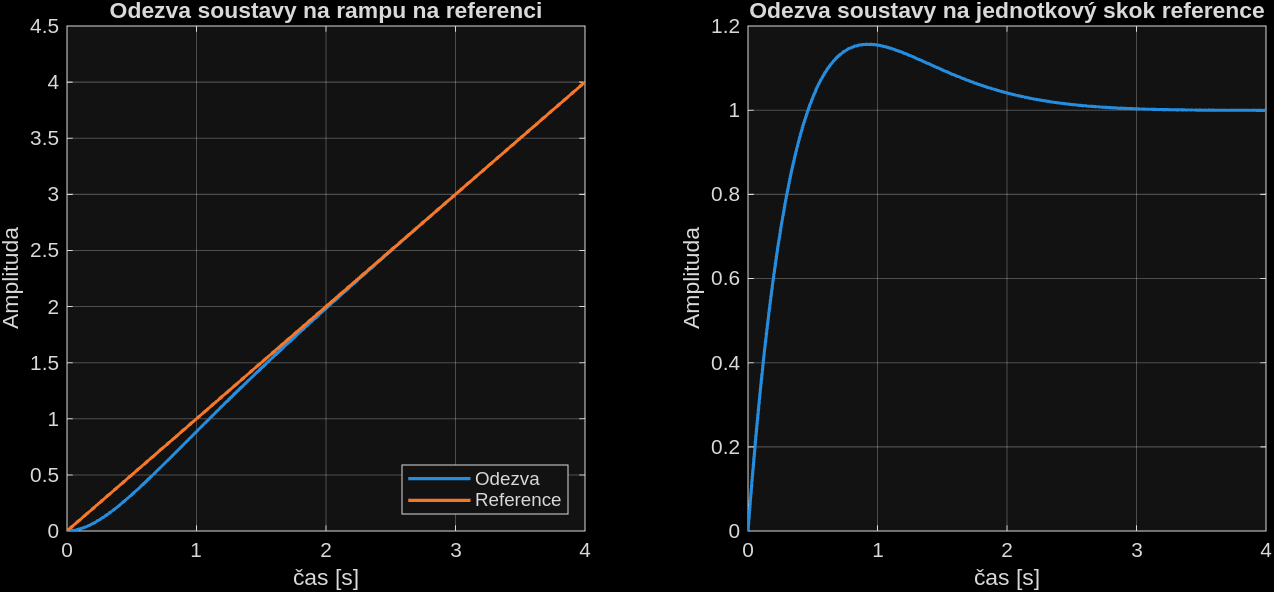
\includegraphics[width=1\textwidth]{graphs.png}
  \caption{grafy}
\end{figure}

\end{document}